\documentclass[aspectratio=169,t]{beamer}
\usepackage[utf8]{inputenc}
\usepackage[T1]{fontenc}


\title{Mobile Anwendungen im Gesundheitswesen}
\date{WS 2019/2020}
\author[PWD]{Prof. Dr.-Ing. Piotr Wojciech Dabrowski}
\titlegraphic{Bilder/logo.png}
% https://pxhere.com/en/photo/1441931

\usepackage{HTWBeamerTemplate/beamerthemeHTW}
\subtitle{0: Allgemeines}
\addbibresource{Bilder/imagesources.bib}
\begin{document}

\setbeamertemplate{footline}[first]
\begin{frame}[noframenumbering]
\titlepage
\end{frame}

\setbeamertemplate{footline}[presentationbody] 

\begin{frame}{Vorstellung}
 \begin{itemize}
     \item<2-> Kurz zu mir
     \only<2-4>{
      \begin{itemize}
        \item<2-4> Kontakt: Piotr.Dabrowski@htw-berlin.de - gerne nutzen!
        \item<2-4> Repository: https://github.com/dabrowskiw/
        \item<3-4> Geboren 1981 in Warschau
        \item<3-4> Studium der Biotechnologie \& Informatik an der TU Berlin
        \item<3-4> Promotion über Auswertung von Hochdurchsatzdaten für Virus-Diagnostik
        \item<3-4> Aufbau der bioinformatischen Analytik für das NGS-Labor des RKI
        \item<3-4> Aufbau der Bioinformatics Core Facility am RKI
        \item<4> Hang zu unkonventionellen Vorlesungsmethoden - Feedback erwünscht!
      \end{itemize}
     }
     \note<4->{Erstes Mal Vorlesung, Background nicht in mobilen Applikationen\\
     Bitte um Geduld, Hinweise
     }
     \item<5-> Der Todesstern \& (ausgewählte) andere Hilfsmittel
     \item<9-> Sie \& Ihre Vorstellungen, Motivation und Vorkenntnisse
     \only<10->{
       \begin{itemize}
           \item Kommt gleich!
       \end{itemize}
     }
 \end{itemize}
 \only<5-8>{
  \begin{textblock}{15}(2,7)
   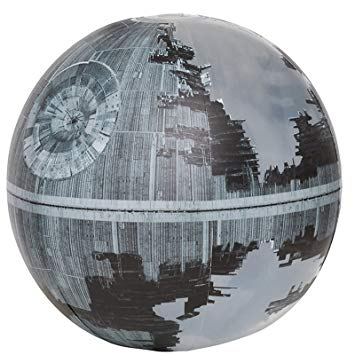
\includegraphics[width=3cm]{Bilder/Todesstern.jpg}
  \end{textblock}
 }
 \only<6-8>{
  \begin{textblock}{15}(5.5,8.25)
   
\includegraphics[width=3cm]{Bilder/Tischnamensschild.png}
  \end{textblock}
 }
 \only<7-8>{
  \begin{textblock}{15}(9,7.5)
   
\includegraphics[angle=77,origin=c,height=2cm]{Bilder/Tischnamensschild.png}
  \end{textblock}
 }
 \only<8>{
  \begin{textblock}{15}(11.5,8)
   
\includegraphics[width=3cm]{Bilder/Whiteboard.png}
  \end{textblock}
 }
\end{frame}

\begin{frame}{Fragen der Vorlesung}
\note{
\begin{itemize}
    \item Entwicklung: Besonders wichtig bei Gesundheitswesen: Stabilität, einfache Anwendbarkeit (patient compliance)
    \item Was sind personenbezogene Daten, wann darf man sie verarbeiten - und wann sollte man sie verarbeiten etc.
\end{itemize}
}
\begin{itemize}
    \item Warum sind mobile Applikationen im Gesundheitswesen sinnvoll? Wo werden sie bereits eingesetzt?
    \item<2-> Worauf muss man bei der Entwicklung mobiler Applikationen für das Gesundheitswesen achten?
    \item<3-> Was sind Herausforderungen im Zusammenhang mit der Verarbeitung potentiell sensitiver Daten?
\end{itemize} 
\end{frame}

\begin{frame}{Inhalt der Übung}
Entwicklung einer mobilen medizinischen Applikation.
    \begin{itemize}
        \item<2-> Zusammenfinden in möglichst balancierten Teams (5 Personen)
        \item<3-> Entwickeln einer Produktidee
        \item<4-> Erstellung eines Mockups
        \item<5-> Implementation eines Proof of Concept
        \item<6-> Erstellung einer Produktpräsentation (15 Minuten/Gruppe)
    \end{itemize}
\end{frame}

\begin{frame}{Benotung}
 \note{
    \begin{itemize}
        \item PoC nicht ``fertig werden'', Idee und Herangehensweise ausschlaggebend.
        \item Produktpräsentation:
        \begin{itemize}
            \item Ideen, Herausforderungen, Umgehen mit Herausforderungen so darstellen, dass sie für die Anderen nachvollziehbar und nützlich sind!
            \item Vorstellung des PoC: Verkaufsevent, warum sind wir besser als alle anderen!
        \end{itemize}
    \end{itemize} 
 }
 \begin{itemize}
     \item<1-> Klausur: $40\%$
     \item<2-> Code- und Repo-Qualität: $40\%$
     \only<3>{
        \begin{itemize}
            \item Dokumentation des Codes (Vorhandensein, Übereinstimmung Dokumentation/Code): $10\%$
            \item Konsistenter Code-Stil: $10\%$
            \item Vorhandensein dokumentierter Tests: $10\%$
            \item Kleinteilige Commits: $10\%$
        \end{itemize}
    }
     \item<4-> Ergebnisvorstellung: $20\%$
     \only<5>{
        \begin{itemize}
            \item 15 Minuten/Gruppe
            \item \textbf{Für alle verständliche} Vorstellung wichtiger Gedanken, Herausforderungen, Entscheidungen, Lösungsansätze
            \item PoC-Präsentation mit Verkaufscharakter: Warum ist/wird das die beste App auf der Welt?
            \item Emfpehlung: Story erzählen.
        \end{itemize}
    }
     \item<6-> Verbesserungsvorschläge/Fehlerkorrekturen
     \only<7>{
         \begin{itemize}
             \item $2.5\%$ pro Stück
    	 \item Maximal 2 pro Semester
    	 \item Wenn als pull request: Doppelte Punktzahl
         \end{itemize}
    }
 \end{itemize}
\end{frame}


\stepcounter{slidesection}
\setbeamertemplate{background}[bgfirst]
\setbeamertemplate{footline}[first]
\subtitle{\theslidesection: Kurzer Einblick in das Gesundheitssystem}
\titlegraphic{Bilder/logo1.png}
\begin{frame}[noframenumbering]
\titlepage
\begin{textblock}{10}(4.75,15)
\cite{GesundheitssystemLogo}
\end{textblock}
\end{frame}
\setbeamertemplate{footline}[presentationbody] 
\setbeamertemplate{background}[bgbody]

\begin{frame}{Begriffsdefinition(en)}
    \begin{definition}
        Das Gesundheitswesen ist die Gesamtheit eines organisierten Handelns als Antwort auf das Auftreten von Krankheit und Behinderung und zur Abwehr gesundheitlicher Gefahren.
    \end{definition}
    \only<2->{\begin{definition}
        Das Gesundheitswesen setzt sich aus allen Instituten, Einrichtungen, Personen und allen Maßnahmen zusammen, die für die Bevölkerung gesundheitsfördernd und -erhaltend sind, vorbeugend gegen Verletzungen und Krankheit wirken sowie diese behandeln.
    \end{definition}}
\end{frame}

\begin{frame}{Akteure im Gesundheitssystem (Überblick)}
   \begin{figure}[h!]
    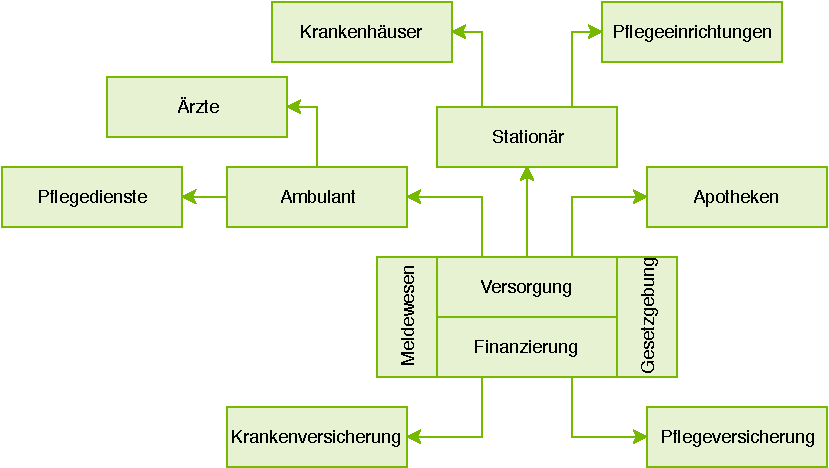
\includegraphics[height=5.5cm]{Bilder/Gesundheitssystem.pdf}
     \caption{Akteure im Gesundheitssystem. Eigene Abbildung in Anlehnung an \cite{SmartHealth}}
   \end{figure}
\end{frame}

\begin{frame}{...und ein kurzer Blick in die Tiefe}
   \begin{figure}[h!]
    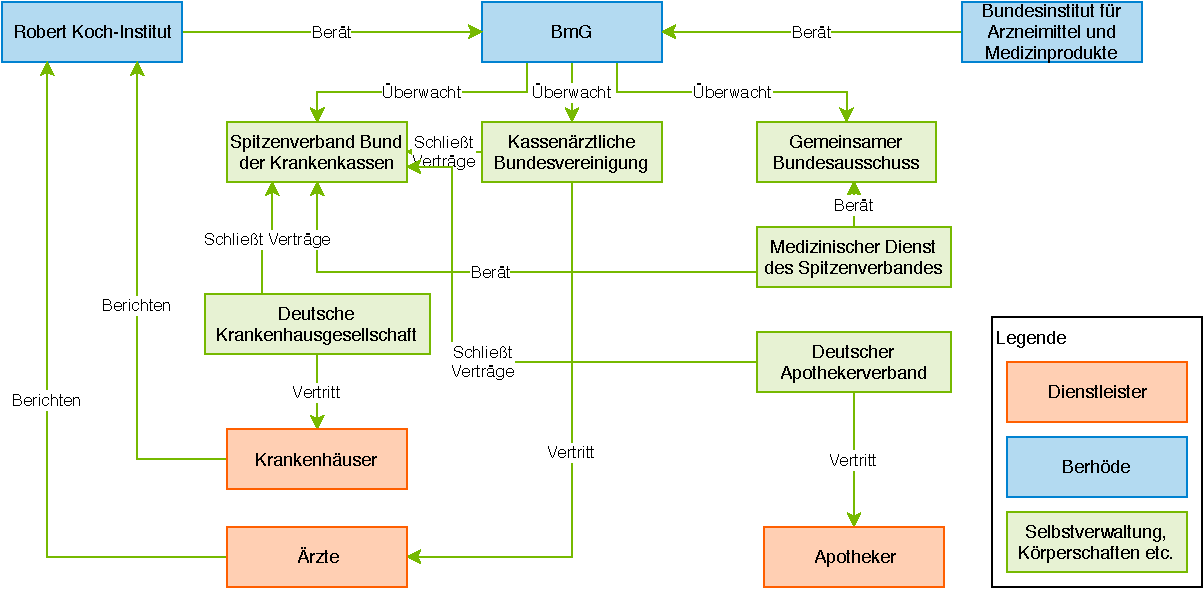
\includegraphics[height=5.5cm]{Bilder/GesundheitssystemAkteureBund.pdf}
     \caption{Einige Interaktionen auf Bundesebene. Eigene Abbildung.}
   \end{figure}
\end{frame}

\begin{frame}{Datenaustausch (Beispiel GKV)}
   \note{\begin{itemize}
       \item Richtlinien für den Datenaustausch im Gesundheits- und Sozialwesen, 110 Seiten
       \item Häufig im Einsatz: Mainframe, COBOL
   \end{itemize}}
   \begin{figure}[h!]
    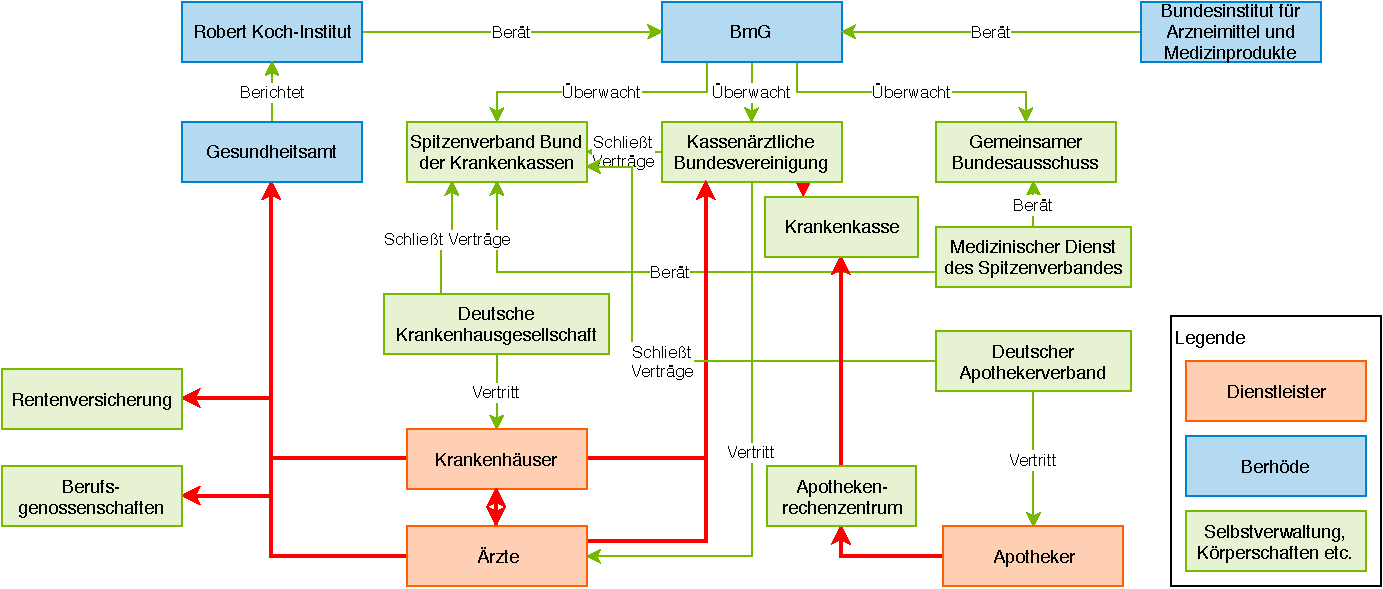
\includegraphics[height=5.5cm]{Bilder/DatenfluesseGesundheitssystem.pdf}
     \caption{Beispiele für Austausch personenbezogener Daten im Gesundheitssystem. Eigene Abbildung.}
   \end{figure}
\end{frame}

\begin{frame}{Herausforderungen}
\note{
\begin{itemize}
    \item Steigende Anzahl an Ärzten
    \item Sinkende Zeit pro Patient
    \item Gründe: 
    \begin{itemize}
        \item Demographischer Wandel
        \item Bessere Behandelbarkeit trivialer Erkrankungen führt zu mehr chronischen und komplexen Erkrankungen
        \item<4> Zunehmende Pflegebedürftigkeit
        \item<4> Steigende Dokumentationspflichten
        \item<4> Steigende Komplexität der Diagnose/Behandlung
    \end{itemize}
\end{itemize}}
\begin{minipage}{.4\textwidth}
   \begin{figure}[h!]
    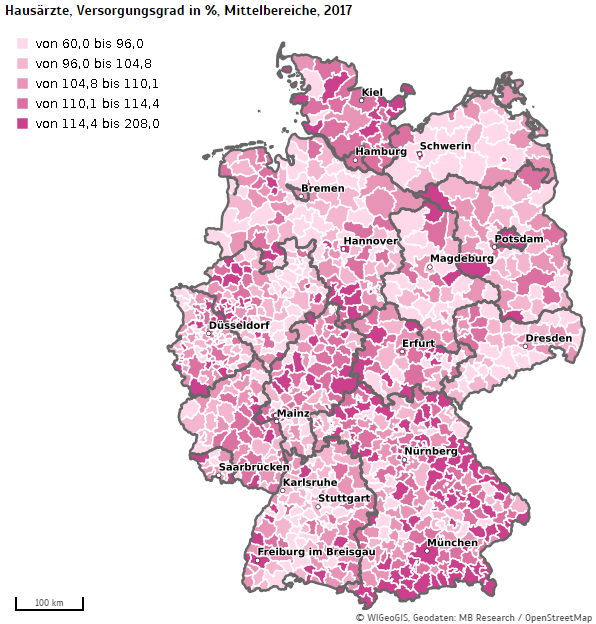
\includegraphics[height=5.5cm]{Bilder/HausarztVersorgung.png}
     \caption{Versorgung mit Hausärzten in 2017 \cite{HausarztVersorgung}}
   \end{figure}
   \end{minipage}
  \only<2->{
  \begin{textblock}{10}(6,0.5)
   \begin{figure}[h!]
     \frame{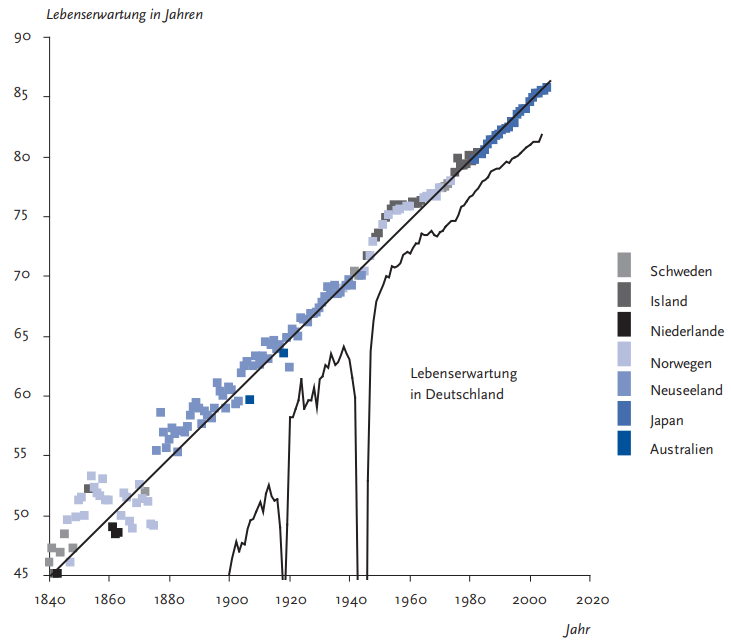
\includegraphics[width=6cm]{Bilder/Rekordlebenserwartungen.PNG}}
     \caption{Anstieg der Rekordlebenserwartung und der Lebenserwartung in Deutschland \cite{GesundheitKrankheitAlter}}
   \end{figure}
  \end{textblock}
  }
  \only<3->{
  \begin{textblock}{10}(6.7,6.7)
   \begin{figure}[h!]
     \frame{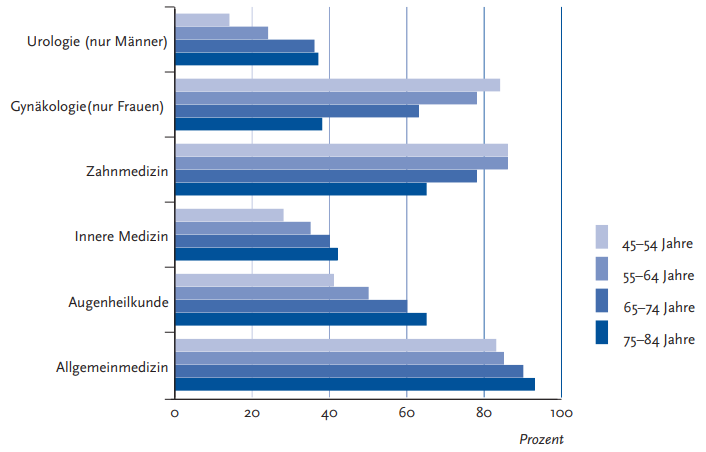
\includegraphics[width=6cm]{Bilder/InanspruchnahmeAerzte.png}}
     \caption{Inanspruchnahme von Ärzten (letzte 12 Monate) nach Alter und Arzt \cite{GesundheitKrankheitAlter}}
   \end{figure}
  \end{textblock}
  }
  \only<4->{
  \begin{textblock}{10}(2.8,3.8)
   \begin{figure}[h!]
     \frame{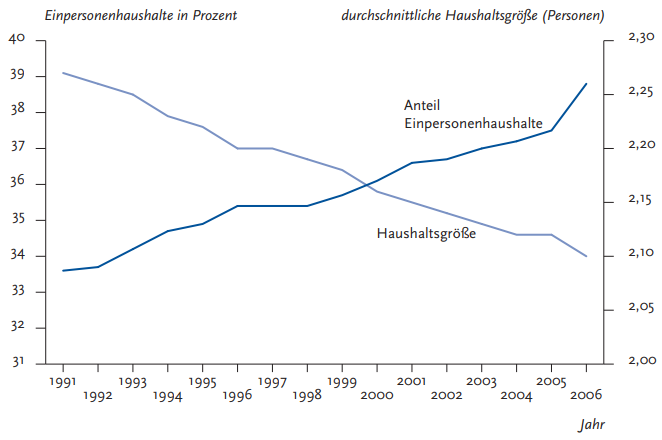
\includegraphics[width=6.5cm]{Bilder/Einpersonenhaushalte.png}}
     \caption{Entwicklung der Haushaltsgröße \cite{GesundheitKrankheitAlter}}
   \end{figure}
  \end{textblock}
 }
\end{frame}

\begin{frame}{IT-Unterstützung}
  \note{
  \begin{itemize}
      \item UC: Z.B. Blutdruck, Blutzucker, Sturzsensor, Lokationssensor (Wandern von Alzheimer-Patienten), Schweiß- und Herzfrequenzüberwachung zur Vorhersage epileptischer Anfälle etc.
      \item Benachrichtigung in Stufen, z.B. Angehörige, dann Pflegepersonal
      \item Erinnerung an Medikamente (Problem: Adhärenz!)
      \item Generell: Ortsunabhängige Pflege (zu Hause)
      \item <2-> Automatische Übertragung von Geräten zu zentralen Datenbanken, automatische Vorauswertungen von Bilddaten
      \item<2-> Standardisierung - großes Problem in Medizintechnik
      \item<3-> Abgleich verschriebener Medikamente mit gelber oder roter Liste
      \item<5-> Automatische Benachrichtigung bei Ablauf von Blutkonserven, RFID-Kennzeichnung von OP-Besteck um Desinfektionszyklen einzuhalten etc.
  \end{itemize}}
  \begin{itemize}
      \item Ubquitous Computing: Sensorik und automatische Benachrichtigungen, insbesondere in der Pflege
      \item<2-> Verbesserung der Technikintegration
      \item<3-> Expertensysteme zur Behandlungsunterstützung
      \item<4-> Dokumentationsunterstützung
      \item<5-> Logistik
      \item<6-> Allgemein: Entlastung und Effizienzsteigerung, um bei gleichem Personal mehr Zeit für die Patienten zu haben
  \end{itemize}
\end{frame}

\begin{frame}{Ihre Vorstellung}
    \note{
        \begin{itemize}
            \item Ziel: Entwicklung einer App im 5er-Team
            \item Manche haben mehr, manche weniger technischen Background
            \item Informationen, um ausgewogene Teams zu erstellen
        \end{itemize}
        Zeit: 10 Minuten. \textbf{Wenn fertig, Namensschild auf Bildschirm!}
    }
    \only<2->{
        Kurzprofil:
        \begin{itemize}
            \item Name
            \item Bisherige Erfahrung (Sprachen, Projekte etc.) in:
            \begin{itemize}
                \item Programmierung
                \item App-Entwicklung
                \item (UI-)Design
            \end{itemize}
            \item Relevante Interessen, idealerweise mit erster App-Idee
        \end{itemize}
    }
    \only<3->{Vorstellung: 2 Minuten + Profilbogen}
\end{frame}

\begin{frame}{Hausaufgabe!}
    Gruppenfindung\only<2->{... oder zumindest schon mal Gedanken machen. }
    \only<3->{
        \begin{itemize}
            \item Auf ausgewogene Teams achten!
            \item Bei Teilteams: Welche Kompetenzen brauchen wir noch?
            \item Erste Ideenabstimmung zum Thema der App
        \end{itemize}
    }
    \only<4->{Nächste Woche ist noch Zeit zum Finalisieren.}
\end{frame}

%\begin{frame}{App-Ideen}
%In der Woche drauf!
%\end{frame}

\stepcounter{slidesection}
\setbeamertemplate{background}[bgfirst]
\setbeamertemplate{footline}[first]
\subtitle{\theslidesection: Technische Grundlagen}
\titlegraphic{Bilder/logo2.png}
\begin{frame}[noframenumbering]
    \titlepage
    \begin{textblock}{10}(4.75,15)
        \cite{ProgrammingLogo}
    \end{textblock}
\end{frame}
\setbeamertemplate{footline}[presentationbody] 
\setbeamertemplate{background}[bgbody]

\begin{frame}{Flutter}
    \note{
        \only<1-2>{
            Wichtig: Keine Werbung für Flutter, zeigt Herangehensweise an neues Projekt (selber keine Erfahrung mit Flutter)
            Beispiele:\\Java super für portable, performante Applikationen, aber mies für Prototyping\\Python super für Prototyping, aber schlecht für Stabilität\\PHP Totalausfall bei Wartbarkeit+Sicherheit, aber toll für schnelle kleine Webapp\\Wünsche JavaScript schnellen und schmerzhaften Tod, setze es trotzdem für interaktive Visualisierungen ein\\etc... \\Fazit: Keine silver bullet, man muss viele Stärken und Schwächen kennen, und z.T. Programmierkonzepte zwischen Sprachen übertragbar. Flexibilität ist wichtig!
        }
        \only<3->{
            Mini-Whiteboard: Was ist wichtig bei der Entscheidung für eine Sprache für ein Projekt?
            \begin{itemize}
                \item Entwickler: Einer? Mehrere? Community oder Spaltungen? Aktivität der Entwicklung? (wikipedia)
                \item Anzahl an reifen Projekten in Sprache (flutter.dev)
                \item Bekannte Schwachstellen und Reaktionen (exploit-db.com, cve.mitre.org etc), konkretes Beispiel: www.cvedetails.com, Oracle (Page 10), Java, Metasploit modules, CVE-2012-4681 Java 7 Applet Remote Code Execution. Google: Page 12. Dart: Dart TCP
                \item Geeignetheit der Features für Problem (bsp. R, shell, PHP)
                \item Verfügbarkeit von relevanten Bibliotheken (pub.dev, chart, flchart)
                \item Verfügbarkeit aktueller Entwicklungstools
                \item Lizenz: Vorhanden? Falls ja, Bedingungen, bsp. GPL vs. LGPL. BSD: Redist license!
            \end{itemize}
        }
    }
    Wichtig in Programmierung: Weniger eine konkrete Sprache, mehr breites Wissen und Verständnis von Konzepten. Also: Richtige Programmiersprache für das Problem wählen! \only<2->{Aber: Was heißt ``richtig?''}\only<4->{\textbf{ Und ist Flutter ``richtig''?}}
    \only<3->{
        \begin{itemize}
            \item[\only<4>{\textbullet}\only<5->{\checkmark}] Aktive Entwicklung
            \item[\only<4-5>{\textbullet}\only<6->{\checkmark}] Starke Aktuere in der Community
            \item[\only<4-6>{\textbullet}\only<7->{\checkmark}] Vorhandensein reifer Produkte
            \item[\only<4-7>{\textbullet}\only<8->{\checkmark}] Sicherheit
            \item[\only<4-8>{\textbullet}\only<9->{\checkmark}] Relevante Bibliotheken und Entwicklungstools
            \item[\only<4-9>{\textbullet}\only<10->{\checkmark}] Bekannte und nutzbare Lizenz
            \item[\only<4-10>{\textbullet}\only<11->{?}] Ausreichende ROI bei fehlenden Vorkenntnissen
        \end{itemize}
    }
\end{frame}

\begin{frame}{Sourcecodeverwaltung}
    \note{
        Bevor wir anfangen, Code zu schreiben, müssen wir uns Gedanken darüber machen, wie wir das tun...
        \begin{itemize}
            \item Perforce
            \begin{itemize}
                \item Einsatz in großen Unternehmen (größtes Repo bei Google, 18/20 top-Spieleherstellern, Netflix etc.)
                \item Ändert darunterliegende Technologie nach Bedarf (aktuell git.kompatibel, aber erste Version 10 Jahre vor git)
            \end{itemize}
            \item Subversion: Tracking von Verschieben, Umbenennen etc.
            \item git: Durch Kommerzialisierung von BitKeeper
            \item mercurial: Gleiches Ziel wie git (Linux-Kernel), heutzutagez.B. bei Facebook und Mozilla im Einsatz
            \item Einer der großen heiligen Kriege: git vs. mercurial
            \item Derzeit primär im Einsatz: SVN, Perforce, TFS (zentral), git, mercurial (dezentral)
        \end{itemize}
    }
    \begin{itemize}
        \item Ursprüngliche Herangehensweise: Datei\_final\_final\_realfinal\_12.java...
        \item<2-> 1972: Bell labs, SCCS (source code control system, single user, nur Textdateien)
        \item<3-> 1986: CVS (concurrent version system, zentral, dateibasiert)
        \item<4-> 1995: Helix core (Perforce)
        \item<5-> 2000: SVN (subversion, zentral, verzeichnisbasiert)
        \item<6-> 2004: TFS (team foundation server, Microsoft, zentral/git, verzeichnisbasiert mit bug tracker etc.)
        \item<7-> 2005: git (Linus Torvalds, dezentral, verzeichnisbasiert)
        \item<8-> 2005: mercurial (dezentral, verzeichnisbasiert)
    \end{itemize}
\end{frame}

\begin{frame}{Sourcecodeverwaltung (git)}
    \note{Abgabe von Übungsaufgaben nur als Release-Link in git-Repository}    
    \begin{minipage}{.4\textwidth}
        \begin{figure}[h!]
            \frame{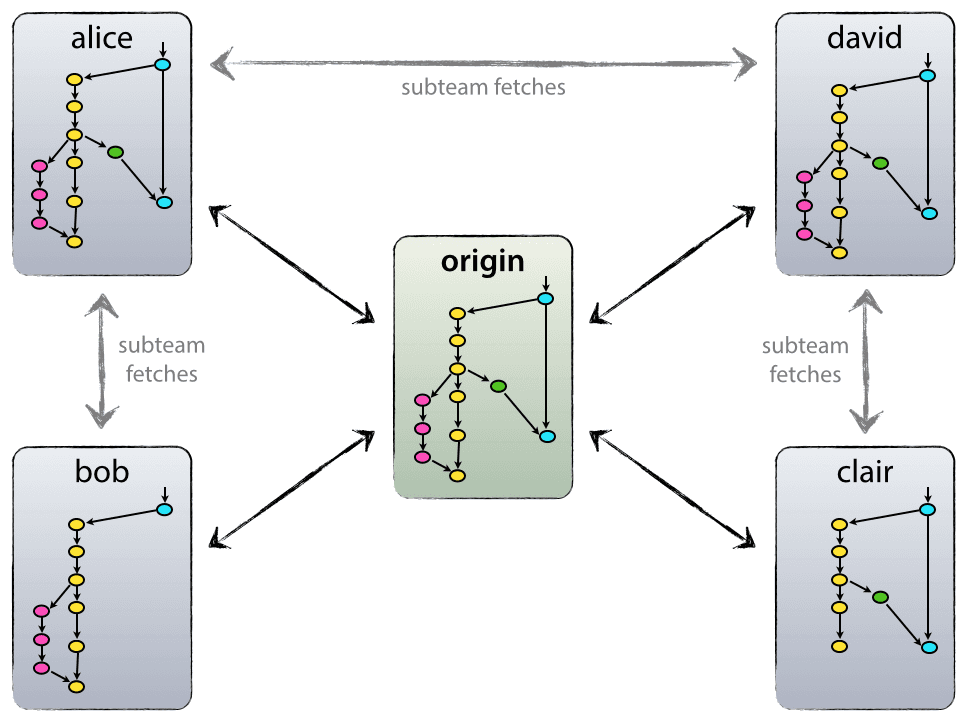
\includegraphics[height=5.5cm]{Bilder/gitbranching2.png}}
            \caption{Teamarbeit mit mehreren remotes \cite{gitbranching}}
        \end{figure}
    \end{minipage}
    \only<2->{
        \begin{textblock}{6}(10,0.2)
            \begin{figure}[h!]
                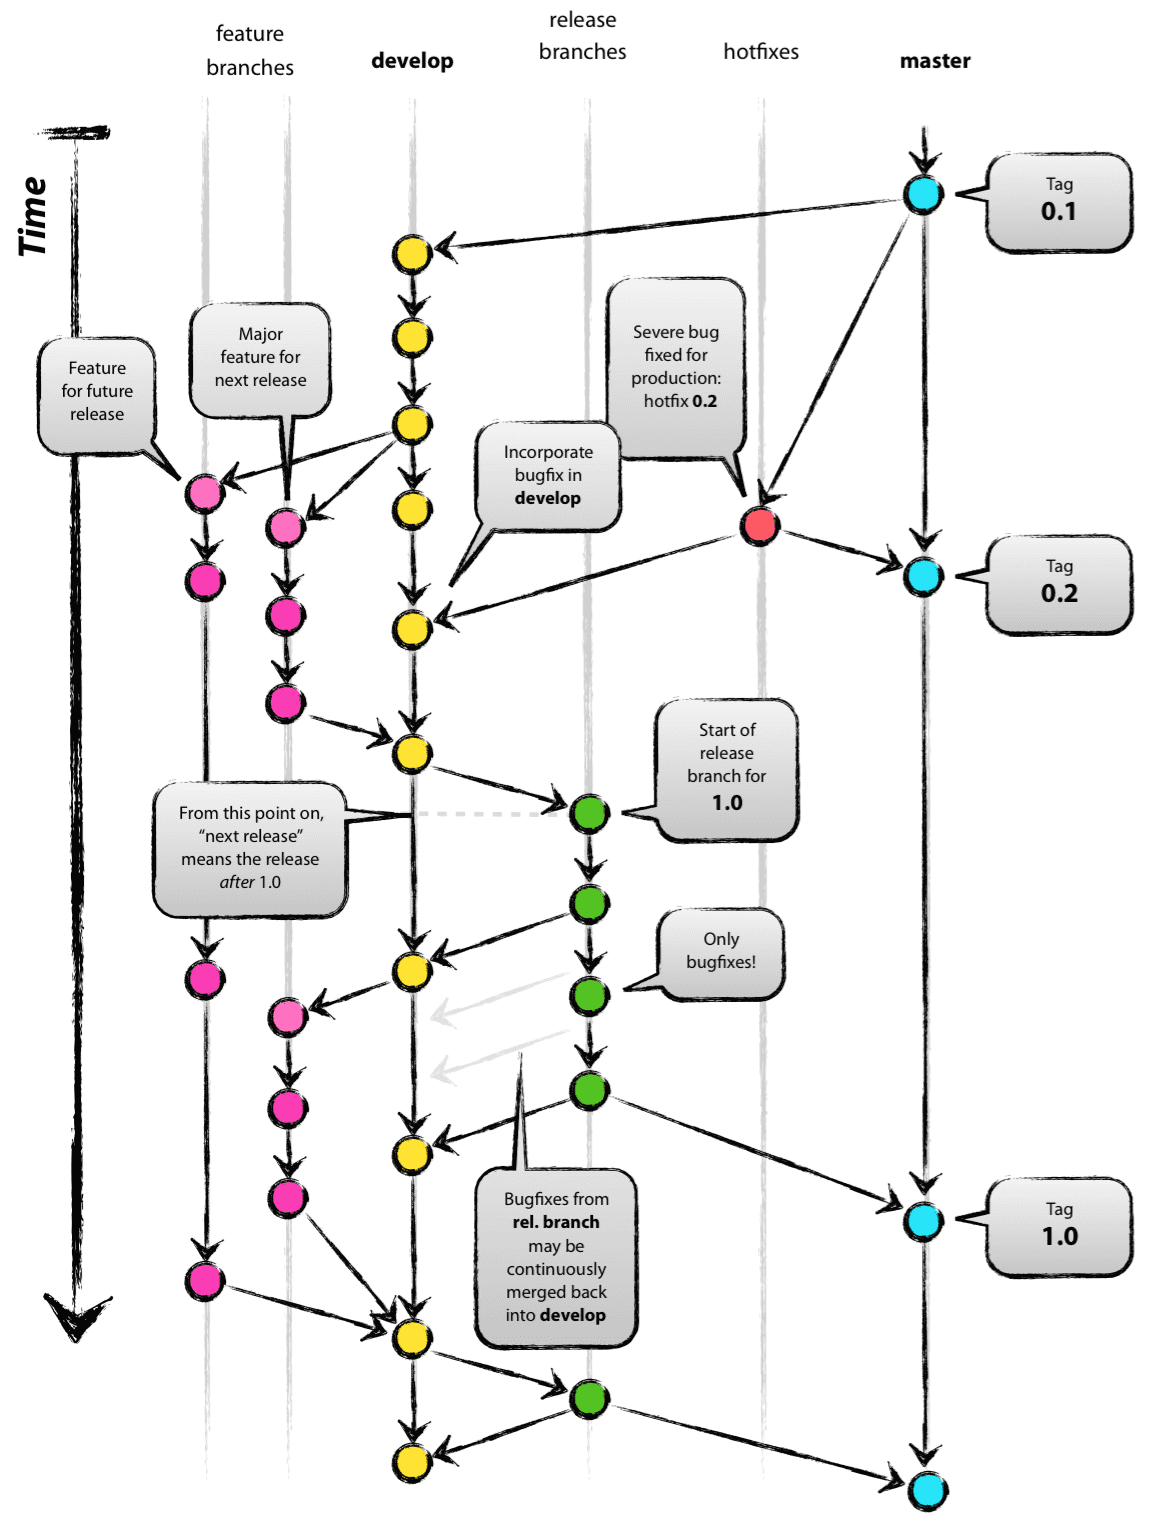
\includegraphics[height=7.3cm]{Bilder/gitbranching.png}
                \caption{Komplexe branching-Strategie \cite{gitbranching}}
            \end{figure}
        \end{textblock}
    }
\end{frame}

\begin{frame}{Übung: git}
    \note{
        \begin{itemize}
            \item Gitlab: Open Source (inhouse betreibbar), kostenfreie private Repositories, einfach konfigurierbares CI/CD. Aber grundsätzlich: Geschmackssache.
            \item<3-> Branch-Anpassung
            \item<5-> Abfrage: Ist .git-credentials ein Problem? Hinweisen auf häufige Wiederverwendung von Mail-Passwort-Kombinationen
            \item<7-> \textbf{Diskutieren}: Passwort für key. Ist passwortloser key besser oder schlechter als .git-credentials? Hinweis auf keepass
            \item<8-> \textbf{Diskutieren}: Ist git push --force nach reset auf gepushten commit  eine gute Idee?
        \end{itemize}
    }
    \begin{itemize}
        \item Erstellung eines gitlab-Accounts
        \item<2-> Neues Projekt erstellen, README anpassen (online)
        \item<3-> clone, README anpassen, commit
        \item<4-> push... Aber wo geht es hin? git remote! Und was geht da hin? git branch
        \item<5-> Credentials merken...
        \item<6-> ...und gleich wieder löschen! 
        \item<7-> Alternative: \href{https://docs.gitlab.com/ee/ssh/}{SSH-Key}. Dafür: clone über SSH (oder remote anpassen?)
        \item<8-> Fehler rückgängig machen: git reset (vor und nach push)
    \end{itemize}
\end{frame}

\begin{frame}{Live-Minimalbeispiel}
\end{frame}


\begin{frame}{Bildquellen}
\printbibliography
\end{frame}

\end{document}
